\documentclass[a4paper,dvipsnames]{article}

\input ../../header

\newcommand{\un}{\left(u_n\right)_{n\in\mathbb{N}}}
\newcommand{\uns}{\left(u_n\right)_{n\in\mathbb{N}^\ast}}
\newcommand{\vn}{\left(v_n\right)_{n\in\mathbb{N}}}
\newcommand{\vns}{\left(v_n\right)_{n\in\mathbb{N}^\ast}}
\newcommand{\wn}{\left(w_n\right)_{n\in\mathbb{N}}}
\newcommand{\wns}{\left(w_n\right)_{n\in\mathbb{N}^\ast}}
\newcommand{\tn}{\left(t_n\right)_{n\in\mathbb{N}}}
\newcommand{\tns}{\left(t_n\right)_{n\in\mathbb{N}^\ast}}
\newcommand{\qn}{\left(q_n\right)_{n\in\mathbb{N}}}
\newcommand{\qns}{\left(q_n\right)_{n\in\mathbb{N}^\ast}}
\newcommand{\N}{\mathbb{N}}

\usepackage{dirtree}
\newcommand{\basthon}[1]{{\href{https://notebook.basthon.fr/?from=#1}{Lien Basthon}}}
\newcommand{\basthonC}[1]{{\href{https://notebook.basthon.fr/?from=#1}{Corrigé}}}

\title{Représentation des caractères}

\author{}
\date{}

\begin{document}

\renewcommand{\contentsname}{}

\pagestyle{fancy}

\begin{tcolorbox}[colframe=blue!75, colback=blue!45, valign=center, height=1.5cm, top=5mm]
  \maketitle
\end{tcolorbox}

\tableofcontents

\vspace{1cm}

\thispagestyle{fancy}

\section{Introduction}

Un ordinateur ne manipule que des $0$ et des $1$ : comment le texte est-il codé ? Puisqu'un texte est une suite de caractères, on va s'intéresser à la représentation des caractères, c'est-à-dire au codage des lettres minuscules et capitales, des chiffres, des signes de ponctuation et autres symboles. Le principe est le suivant :

\begin{itemize}
  \item Chaque caractère est identifié par un code unique qui est un entier naturel. La correspondance entre le caractère et son code est appelé un \textbf{Charset}.
  \item Le code n'étant pas utilisable tel quel par un ordinateur qui ne comprend que le binaire, il faut donc représenter les codes par des octets : c'est l'\textbf{Encoding}.
\end{itemize}

\section{Le code ASCII}

\subsection{Présentation}

Le code ASCII (\textit{American Standard Code for Information Interchange}) définit $128$ caractères numérotés de $0$ à $127$ et codés en binaire de $000\,0000$ à $111\,1111$. Sept bits suffisent donc. Cependant, depuis les années 1970, presque tous les ordinateurs travaillent avec des multiples de huit bits (un octet) : chaque caractère d'un texte en ASCII est souvent stocké sur huit bits, le huitième bit (celui de poids fort) étant égal à $0$. 

\smallskip

Parmi ces $128$ caractères :

\begin{itemize}
  \item $95$ sont imprimables : il s'agit des chiffres de $0$ à $9$, des lettres minuscules et capitales de A à Z, et de symboles mathématiques et de ponctuation ;
  \item les $33$ autres caractères (les caractères de numéro $0$ à $31$ et le $127$) ne sont pas affichables : ils correspondent à des commandes de contrôle de terminal informatique. Par exemple, le caractère numéro $127$ est la commande pour effacer. Le caractère numéro $32$ est l'espace. Le caractère numéro $7$ provoque l'émission d'un signal sonore.
\end{itemize}

\begin{center}
  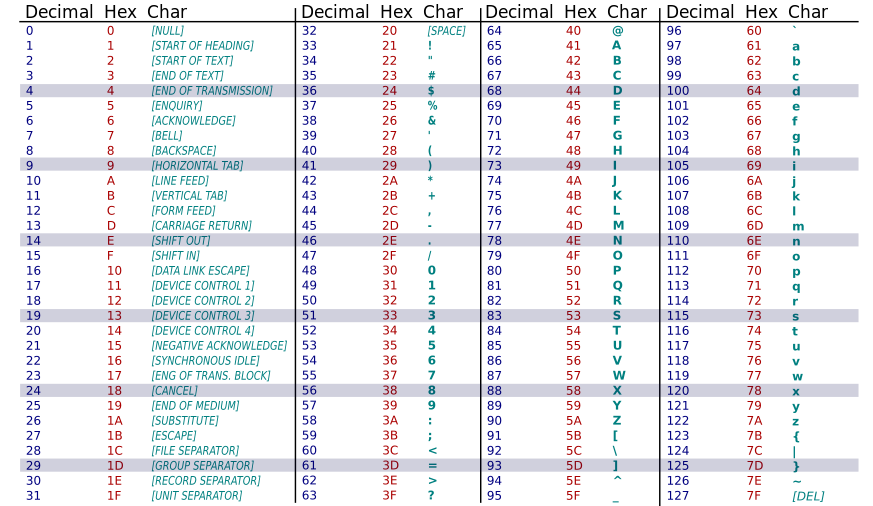
\includegraphics[width=16cm]{img/ascii-table.png}
\end{center}

\medskip

\begin{exercice}{}{}
  \begin{enumerate}
    \item Quel nombre suffit-il d'ajouter au code d'une lettre capitale pour obtenir la lettre minuscule correspondante ?
    \item En pratique, que suffit-il de changer à l'écriture binaire de ce code ?
  \end{enumerate}
\end{exercice}

\medskip

On peut représenter cette table sous une forme plus condensée en ne donnant que l'Encoding (ici en hexadécimal) :

\begin{center}
  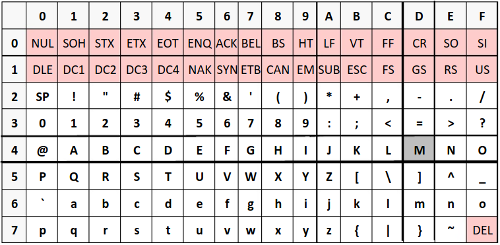
\includegraphics[width=13cm]{img/ascii-table-hexa-encoding.png}
\end{center}

\medskip

\begin{activite}[breakable]{taille d'un texte}{}
  \begin{enumerate}
    \item Donner la taille (en octets) de la phrase suivante (sans les guillemets) : \og{}La NSI, c'est chouette !\fg{}
    \item Écrire cette phrase dans un fichier \verb|chouette| :
      \begin{itemize}
        \item Créer un fichier \verb|chouette| vide à l'aide de la commande \verb|vim chouette|.
	\item Passer en mode insertion en appuyant sur \verb|i|, puis saisir la phrase \og{}La NSI, c'est chouette !\fg{}.
	\item Appuyer sur la touche \verb|ESC| pour sortir du mode insertion (on est alors dans le mode normal de Vim).
	\item Sauvegarder les modifications faites en appuyant sur \verb|:w| suivi de \verb|Entrée|.
	\item Quitter Vim à l'aide de \verb|:q| suivi de \verb|Entrée|.
      \end{itemize}
    \item Quelle commande permet de connaître la taille du fichier \verb|chouette| ? Vérifier que le résultat obtenu est cohérent avec la taille déterminée à la question 1.
    \item  Écrire maintenant la même phrase dans le logiciel de traitement de texte \verb|LibreOffice Writer|.
      \begin{itemize}
        \item Quelle est la taille du fichier obtenu ?
	\item Quelles peuvent en être les explications ?
      \end{itemize}
  \end{enumerate}
\end{activite}

\medskip

\begin{activite}{utilisation de la table ASCII}{}
  \begin{enumerate}
    \item Coder en binaire le mot "Orwell".
    \item Voici maintenant une phrase codée en binaire : 
      \[01010111\ \ 01100001\ \ 01110010\ \ 00100000\ \ 01101001\ \ 01110011\] 
      \[00100000\ \  01010000\ \ 01100101\ \ 01100001\ \ 01100011\ \ 01100101\ \ 00101110\] 
      La retrouver.
    \item Vérifier vos réponses sur \url{https://mothereff.in/binary-ascii}.
    \item Peut-on coder en binaire la phrase \og{}L’Histoire était récrite, mais des fragments de la littérature du passé survivraient çà et là, imparfaitement censurés et, aussi longtemps que l’on gardait l’ancilangue, il était possible de les lire.\fg{} ?  
  \end{enumerate}
\end{activite}

\subsection{Limitations}

Le code ASCII  a d'abord été conçu pour des textes écrits en anglais. Il n'est pas adapté pour représenter des textes écrits dans d'autres langues, mêmes celles qui, comme le français, utilisent l'alphabet latin, car ces langues utilisent par exemple des accents, des cédilles etc. Il a donc fallu étendre la table ASCII pour pouvoir coder les nouveaux caractères, en utilisant le 8\ieme{} bit.

\medskip

\begin{exercice}{}{}
  Combien de nouvelles possibilités l'utilisation du 8\ieme{} bit engendre-t-elle ?
\end{exercice}

\section{Premières extensions de la table ASCII}

La norme ISO 8859-1 (appelée aussi Latin-1 ou Europe occidentale), dont le nom complet est ISO/CEI 8859-1, est une des premières extensions de la table ASCII. Elle a été conçue dans les années 1980 et permet de coder 191 caractères de l'alphabet latin qui avaient à l'époque été jugés essentiels dans l'écriture, mais omet quelques caractères fort utiles (comme la ligature \oe).

\smallskip

Cette norme est très utilisée dans les pays occidentaux et a donné lieu à quelques extensions et adaptations dont Windows-1252 et ISO 8859-15. Ces deux extensions prennent notamment en compte la ligature \oe et le symbole €.

\smallskip

Voici deux tableaux présentant côte à côte ces deux extensions :

\begin{center}
  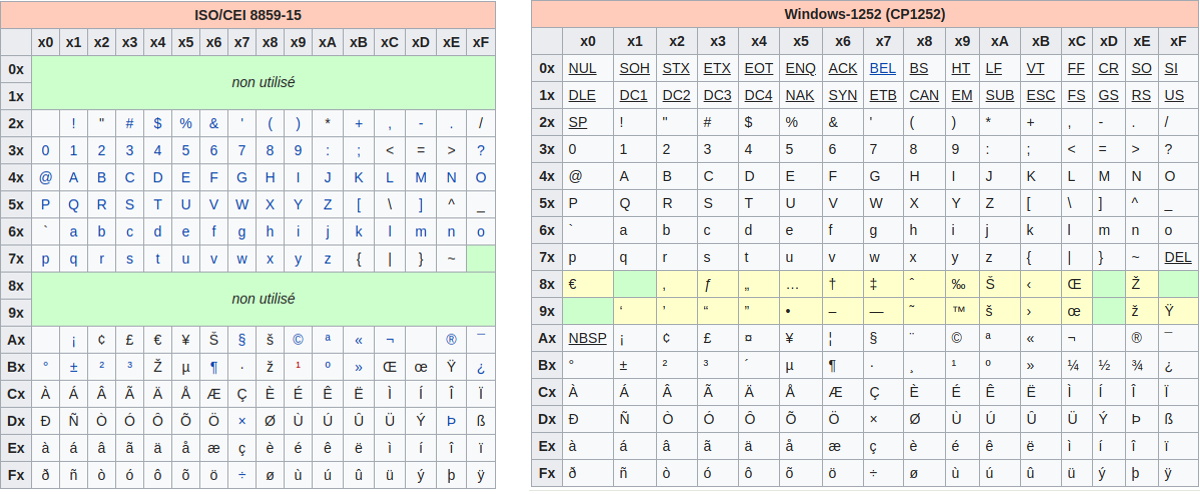
\includegraphics[width=17cm]{img/extensions.png}
\end{center}

\medskip

\begin{exercice}{}{}
  Ces deux extensions sont-elles compatibles ?
\end{exercice}

\section{Unicode}

\subsection{Bizarre ?}

À qui n'est-il pas arrivé de lire un texte telle que celui-ci ?

\begin{quote}
  Il était entendu que lorsque le novlangue serait une fois pour toutes adopté et que l'ancilangue serait oublié, une idée hérétique – c'est-à -dire une idée s'écartant des principes de l'angsoc – serait littéralement impensable, du moins dans la mesure où la pensée dépend des mots.
\end{quote}

Bien que ceci soit de moins en moins fréquent, on trouve parfois des phrases dans lesquelles certains caractères sont remplacés par d'autres qui n'ont rien à voir et qui rendent difficiles voire empêchent la lecture et la compréhension du texte. Il s'agit ici d'un problème d'encodage et de décodage : la personne qui a écrit le texte utilise une norme différente de celle qu'utilise la personne qui le lit.

\subsection{La norme Unicode}
La globalisation des échanges culturels et économiques ainsi que la généralisation de l'utilisation d'Internet ont rendu nécessaire la prise en compte d'un nombre beaucoup plus important de caractères. La norme Unicode a donc été créée pour permettre des échanges de textes dans différentes langues, à un niveau mondial.

\smallskip

Unicode est une table de correspondance Caractère-Code (Charset) : cette table permet d'associer à chaque caractère un nom et un \og{}numéro\fg{} unique appelé \og{}point de code\fg{} (\textit{code point}). Par exemple, le point de code \verb|U+0041| est associé à la lettre \verb|A|. Le \verb|U+| signifie \og{}Unicode\fg{}, et la suite (\verb|0041|) est un nombre écrit en hexadécimal.

\medskip

\begin{exercice}{}{}
  À quelle chaîne de caractères correspond la suite de points de code ci-dessous ?

  \begin{center}
    \verb|U+0057| \verb|U+0069| \verb|U+006E| \verb|U+0073| \verb|U+0074| \verb|U+006F| \verb|U+006E|
  \end{center}

  On pourra consulter avec profit le document \og{}Basic Latin (ASCII)\fg{} disponible \href{http://www.unicode.org/charts/}{ici}.
\end{exercice}

\medskip

\begin{exercice}{}{}
  Reprendre le deuxième tableau de cette fiche, et vérifier l'affirmation précédente.
\end{exercice}

\medskip

\begin{activite}{}{}
  \begin{enumerate}
    \item En utilisant Firefox, aller sur la page internet suivante : 

      \begin{center}
        \url{https://fr.wikipedia.org/wiki/1984_(roman)}.
      \end{center}

    \item Afficher le code source de la page (clic-droit suivi de \textit{Code source de la page} ou avec le raccourci clavier \verb|Ctrl+U|).
    \item Quel est l'encodage défini dans l'en-tête du fichier html ?
    \item Sauvegarder la page puis changer l'encodage précédent et le remplacer par \verb|ISO-8859-1|.
    \item Afficher la page modifiée à l'aide de Firefox : que constate-t-on ?
  \end{enumerate}
\end{activite}

\subsection{Notions d'UTF-8}

Pour encoder les caractères Unicode, UTF-8 utilise un nombre variable d'octets :

\begin{center}
  \small
  \begin{tabular}{@{}cccccc@{}}
    \textbf{1\ier{} octet} & \textbf{2\ieme{} octet} & \textbf{3\ieme{} octet} & \textbf{4\ieme{} octet} & \textbf{Nombre de bits} & \textbf{Point de code}\\
    \midrule
    ${\color{red}0}\text{xxxxxxx}$ & & & & $7$ & jusqu'à 007F ($127)$\\
    ${\color{red}110}\text{xxxxx}$ & ${\color{red}10}\text{xxxxxx}$ & & & $5+6=11$ & de 0080 à 07FF (de $128$ à $\np{2047}$)\\
    ${\color{red}1110}\text{xxxx}$ & ${\color{red}10}\text{xxxxxx}$ & ${\color{red}10}\text{xxxxxx}$ & & $4+6+6=16$ & de 0800 à FFFF (de $\np{2048}$ à $\np{65535}$\\
    ${\color{red}11110}\text{xxx}$ & ${\color{red}10}\text{xxxxxx}$ & ${\color{red}10}\text{xxxxxx}$ & ${\color{red}10}\text{xxxxxx}$ & $3+6+6+6=21$ & de 10000 à 10FFFF (de $\np{65536}$ à $\np{1114111}$)\\
    \bottomrule
  \end{tabular}
\end{center}

\medskip

\begin{remarque}{}{}
  Le nombre de $1$ consécutifs du premier octet est égal au nombre d'octets nécessaires.
\end{remarque}

\medskip

\begin{activite}{}{}
  \begin{enumerate}
    \item Déterminer le point de code du caractère \verb|é| en utilisant ce \href{https://unicode.org/charts/PDF/U0080.pdf}{document}. Combien d'octets sont nécessaires pour l'encoder en utilisant UTF-8 ? Déterminer cet encodage.
    \item  En quoi le codage binaire du \verb|é| peut-il être décodé si on se trompe d'encodage et qu'on utilise par exemple la norme ISO 8859-1 ?
    \item Vérifier votre réponse à l'aide du texte du paragraphe 4.1.
    \item  Il reste des caractères étranges dans le texte : ``ù``. Comment retrouver la signification de ces caractères ?
  \end{enumerate}
\end{activite}

\end{document}
